\documentclass[tikz,border=8pt]{standalone}
\usetikzlibrary{arrows.meta,calc,decorations.markings}

% Tweak wireframe density/height if you like
\def\nrings{5}     % number of horizontal ellipses (z-slices)
\def\rmax{2.2}     % radius of largest ellipse (floor)
\def\zmax{2.9}     % max plotted height

\begin{document}
	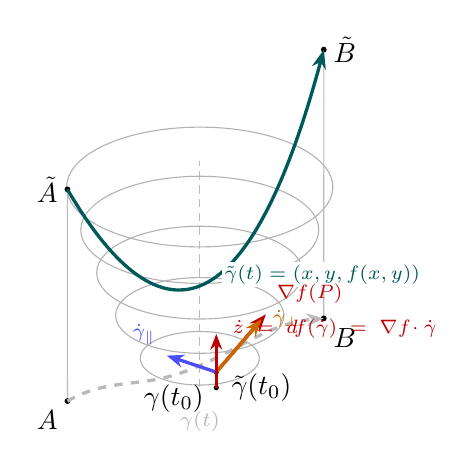
\begin{tikzpicture}[scale=1.05, >=Stealth,
		axis/.style={->, thick},
		labelbox/.style={draw, rounded corners, fill=white, inner sep=2pt, font=\scriptsize},
		lift/.style={very thick, teal!70!black},
		floorcurve/.style={very thick, gray!55, dashed}]
		
%		% ---------- Oblique axes (simple 3D look) ----------
%		\draw[axis] (0,0) -- (4.2,0) node[below right] {$x$};
%		\draw[axis] (0,0) -- ++(-2.3,1.3) node[left] {$y$};  % oblique y
%		\draw[axis] (0,0) -- (0,3.6) node[above] {$z$};
%		
%		% ---------- Floor (z=0) reference ellipse ----------
%		\draw[gray!40] (0,0) ellipse [x radius=\rmax, y radius=0.9];
		
		% ---------- Paraboloid wireframe: z = x^2 + y^2 ----------
		\foreach \k in {1,...,\nrings}{
			\pgfmathsetmacro{\zz}{\k*\zmax/(\nrings+0.6)}
			\pgfmathsetmacro{\rx}{sqrt(\zz)}      % x-radius
			\pgfmathsetmacro{\ry}{0.45*sqrt(\zz)} % squashed y-radius for perspective
			\draw[gray!60] (0,\zz) ellipse [x radius=\rx, y radius=\ry];
		}
		\draw[gray!55, densely dashed] (0,0) -- (0,\zmax); % central spine
		
		% ---------- Endpoints on the floor ----------
		\coordinate (Axy) at (-1.6,0.0);
		\coordinate (Bxy) at ( 1.5,1.0);
		
		% Lift endpoints to the surface: z = x^2 + y^2
		\pgfmathsetmacro{\Az}{(-1.6)*(-1.6) + (0.0)*(0.0)}
		\pgfmathsetmacro{\Bz}{(1.5)*(1.5) + (1.0)*(1.0)}
		\coordinate (A) at ($(Axy)+(0,\Az)$);  % (x,z) in this oblique view
		\coordinate (B) at ($(Bxy)+(0,\Bz)$);
		
		% Vertical projection lines and markers
		\draw[gray!55] (Axy) -- (A);
		\draw[gray!55] (Bxy) -- (B);
		\fill (Axy) circle (1.0pt) node[below left] {$A$};
		\fill (Bxy) circle (1.0pt) node[below right] {$B$};
		\fill (A)   circle (1.0pt) node[left]       {$\tilde A$};
		\fill (B)   circle (1.0pt) node[right]      {$\tilde B$};
		
		% ---------- Base curve gamma on the floor ----------
		\draw[floorcurve, -{Stealth[length=2.2mm]}]
		(Axy) to[out=30,in=200] (-0.2,0.35)
		to[out=20,in=185] (Bxy)
		node[midway, below=2pt, fill=white, inner sep=1pt, font=\scriptsize] {$\gamma(t)$};
		
		% ---------- Pick two intermediate floor control points and lift them ----------
		% Control point C on the floor and its height
		\pgfmathsetmacro{\Cx}{-0.2} \pgfmathsetmacro{\Cy}{0.35}
		\pgfmathsetmacro{\Cz}{\Cx*\Cx + \Cy*\Cy}
		\coordinate (Cxy) at (\Cx,\Cy);
		\coordinate (C)   at (\Cx,\Cz);  % (x,z)
		
		% Control point D on the floor and its height
		\pgfmathsetmacro{\Dx}{0.8} \pgfmathsetmacro{\Dy}{1.0}
		\pgfmathsetmacro{\Dz}{\Dx*\Dx + \Dy*\Dy}
		\coordinate (Dxy) at (\Dx,\Dy);
		\coordinate (D)   at (\Dx,\Dz);  % (x,z)
		
%		% (Optional) draw vertical connectors for control points (guides)
%		\draw[gray!50, densely dashed] (Cxy) -- (C);
%		\draw[gray!50, densely dashed] (Dxy) -- (D);
		
		% ---------- Lifted curve \tilde\gamma on the surface ----------
		\draw[lift, -{Stealth[length=2.4mm]}]
		(A) .. controls (C) and (D) .. (B)
		node[midway, right=1pt, fill=white, inner sep=1pt, font=\scriptsize]
		{$\tilde\gamma(t)=(x,y,f(x,y))$};
		
		% ---------- A sample point P and vertical speed label ----------
		\pgfmathsetmacro{\Px}{0.2} \pgfmathsetmacro{\Py}{0.35}
		\pgfmathsetmacro{\Pz}{\Px*\Px + \Py*\Py}
		\coordinate (Pxy) at (\Px,\Py);
		\coordinate (P)   at (\Px,\Pz);
		\draw[gray!55, densely dashed] (Pxy) -- (P);
		\fill (Pxy) circle (0.9pt) node[below left, yshift=-1pt, xshift=-1pt] {$\gamma(t_0)$};
		\fill (P)   circle (0.9pt) node[right, xshift=2pt] {$\tilde\gamma(t_0)$};
		
		% Planar gradient and velocity split (schematic)
		\draw[red!75!black, very thick, -{Stealth[length=2.2mm]}]
		(Pxy) -- ($(Pxy)+(0.6,0.7)$) node[above right, font=\scriptsize] {$\nabla f(P)$};
		\draw[blue!70, very thick, -{Stealth[length=2.2mm]}]
		(Pxy) -- ($(Pxy)+(-0.6,0.20)$) node[above left, font=\scriptsize] {$\dot\gamma_\parallel$};
		\draw[orange!80!black, very thick, -{Stealth[length=2.2mm]}]
		(Pxy) -- ($(Pxy)+(0.55,0.64)$) node[right, font=\scriptsize] {$\dot\gamma_\perp$};
		
		% Vertical speed at lifted point
		\draw[red!75!black, very thick, -{Stealth[length=2mm]}]
		(P) -- +(0,0.65)
		node[right, font=\scriptsize, xshift=2pt, yshift=2pt]
		{$\dot z \;=\; df(\dot\gamma)\;=\;\nabla f\!\cdot\dot\gamma$};
		
%		% ---------- Integral statement & function label ----------
%		\node[labelbox, anchor=north west] at (-2.5,3.5)
%		{$\displaystyle \int_\gamma df \;=\; \int \dot z\,dt \;=\; f(B)-f(A)$};
%		\node[labelbox, anchor=north east] at (4.2,0.1)
%		{$z=f(x,y)=x^2+y^2$};
		
	\end{tikzpicture}
\end{document}
